\documentclass[a4paper,12pt]{article}

\usepackage{amsmath,amssymb,amsthm,tikz}
\usetikzlibrary{calc,arrows.meta}
\usepackage[margin=20mm]{geometry}
\usepackage{hyperref}

\setlength{\parindent}{0pt}
\setlength{\columnsep}{1cm}

\begin{document}

\twocolumn

\thispagestyle{empty}

\begin{center}
{\Large Assignment 12}\\
{\Large Published on 2020-12-06,}\\
{\em Estimated Time: 30 minutes,}\\
{\em Max.grade 10\textperthousand} 
\end{center}


\section{Strongly Connected Components}

One of the multiple practical applications of a DFS traversal of a directed graph
is finding strongly connected components (strongly connected graphs are defined 
in (Goodrich2011, p.626)), the relevant algorithm is 
known as Kosaraju's algorithm. 
See \url{https://bit.ly/3lI20ec}, \url{https://bit.ly/3mNU2la}. 

{\bf Definition.} A subset of vertices in a directed graph $S \subseteq G.V$ makes a strongly 
connected component, iff for any two distinct vertices $u,v$ there is 
a path $u \leadsto v$ (one or more  and also another path $v \leadsto u$ that goes 
back from $v$ to $u$).

If you can travel only in one direction (say, from $u$ to $v$), but cannot return, 
then $u,v$ should be in different strongly connected components.
(Same thing, if $u$ and $v$ are mutually unreachable.) Moreover, every 
vertex is strongly connected to itself \textendash{} so even in the worst case
a graph with $n$ vertices would have at most $n$ strongly connected components 
(containing one vertex each). 

Figure~\ref{fig:strongly-connected-transposed} shows an example of a graph with $n=5$ vertices
having $3$ strongly connected components. Next to that graph is the {\em transposed graph} $G^T$
where all the edges are reversed.

\begin{figure}[!htb]
\center{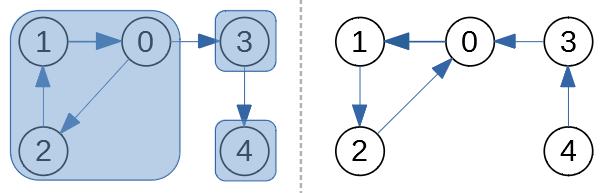
\includegraphics[width=3in]{assignment12-strongly-connected/strongly-connected-transposed.png}}
\caption{\label{fig:strongly-connected-transposed} Graph $G$ and $G^T$}
\end{figure}

\subsection{Kosaraju's algorithm} 

There is a way to find strongly connected components in an 
arbitrary graph by 
running DFS twice (i.e. it works in linear time $O(n+m)$). 


$$\begin{array}{rl}
  & \text{\sc Strongly\textunderscore{}Connected}(G)\\
  & \textcolor{teal}{\text{\em (compute all finishing times $u.f$)}}\\
1 & \text{call}\;\text{\sc DFS}(G)\\
  & \textcolor{teal}{\text{\em ($G^T$ is transposed $G$, all edges reversed)}}\\
2 & \text{compute}\;G^{T}\\
  & \textcolor{teal}{\text{\em (visit vertices in decreasing $u.f$ order)}}\\
3 & \text{call}\;\text{\sc DFS}(G^T)\\
4 & \text{\bf for each}\;\text{tree $T$ in the forest}\;\text{\sc DFS}(G^T)\\
5 & \hspace{0.5cm} \text{Output $T$ as a component}\\
\end{array}$$

To see how this works, we can run it on the example graph shown earlier. 
After the DFS on graph $G$ is run, we get the finishing times 
for the vertices $0,1,2,3,4$ (all shown in red on the left side 
of Figure~\ref{fig:strongly-connected-dfs}.). 
After that we replace $G$ by $G^T$ (to the right side of 
the same figure), and assign priorities in the decreasing sequence
of $u.f$ (the finishing times when running $\text{\sc DFS}(G)$). 

\begin{figure}[!htb]
\center{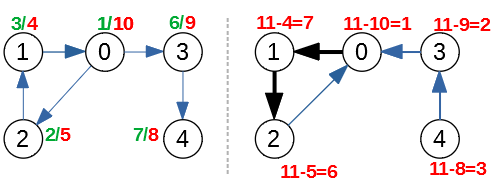
\includegraphics[width=3in]{assignment12-strongly-connected/strongly-connected-dfs.png}}
\caption{\label{fig:strongly-connected-dfs} DFS on $G$ and $G^T$}
\end{figure}


To make this reverse order obvious, we assign new priorities to 
the vertices in $G^T$. The new priorities in $G^T$ are the following:

\begin{itemize}
\item Vertex {\tt "0"} has priority $11 - 10 = 1$.
\item Vertex {\tt "1"} has priority $11 - 4 = 7$. 
\item Vertex {\tt "2"} has priority $11 - 5 = 6$. 
\item Vertex {\tt "3"} has priority $11 - 9 = 2$. 
\item Vertex {\tt "4"} has priority $11 - 8 = 3$. 
\end{itemize}

Now run $\text{\sc DFS}(G^T)$. It turns out that the DFS algorithm starts
in the vertex {\tt "0"} once again (since it was finished last in $\text{\sc DFS}(G)$). 
But unlike the DFS algorithm in $G$ itself (it produced just one DFS tree), 
we get a DFS forest with 3 components (tree/discovery edges shown bold and black in
Figure~\ref{fig:strongly-connected-dfs}). 

\begin{itemize}
\item $\{ \mathtt{"0"}, \mathtt{"1"}, \mathtt{"2"} \}$ (DFS tree has root $\mathtt{"0"}$).
\item $\{ \mathtt{"3"} \}$ (DFS tree has root $\mathtt{"3"}$).
\item $\{ \mathtt{"4"} \}$ (DFS tree has root $\mathtt{"4"}$).
\end{itemize}

They represent the strongly connected components in $G$ (they are also 
strongly connected in $G^T$). 



\section{Problem}

We start with the graph shown in Figure~\ref{fig:problem-graph}.

\begin{figure}[!htb]
\center{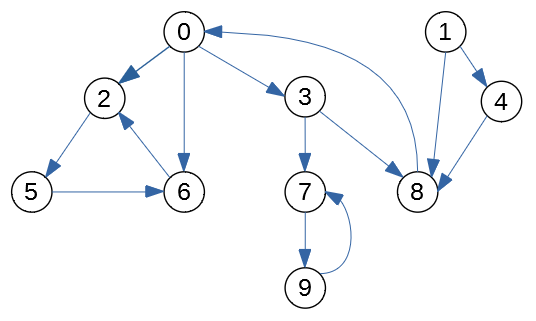
\includegraphics[width=3in]{assignment12-strongly-connected/problem-graph.png}}
\caption{\label{fig:problem-graph} Graph diagram}
\end{figure}

\vspace{10pt}
{\bf (A)} Compute the following three numbers from $a,b,c$ (your last 
Student ID numbers): 
$$\left\{ \begin{array}{l}
U = 2 \cdot ((a+b)\;\text{mod}\;5)\\
V = 2 \cdot ((b+c)\;\text{mod}\;5)+1\\
W = 2 \cdot ((c+a)\;\text{mod}\;5)+1\\
\end{array} \right.$$

By $(x\;\text{mod}\;y)$ we denote the remainder as $x$ is divided by $y$. 
Add to the original graph two new directed edges $(U,V)$ and $(U,W)$. 
(For example, if $U = 2$, $V = 7$, $W = 1$ then add two outgoing edges from 
{\tt "2"} to {\tt "5"} and {\tt "1"} respectively. If an edge exists, do 
not add anything.)

Draw the new graph; show the newly added edges in bold or colored differently.

\vspace{10pt}
{\bf (B)} Run the DFS traversal algorithm on the graph $G$. 
Mark each vertex 
with the pair of numbers {\tt d/f}, where the first number {\tt d} is the 
discovery time, and the second number {\tt f} is the finishing time. 

\vspace{10pt}
{\bf (C)} Draw the transposed directed graph (same vertices, but each arrow points
in the opposite direction). 
Run the DFS traversal algorithm on $G^T$. Make sure that the DFS 
outer loop visits the vertices in the reverse order by $u.f$ 
(the finishing time for the DFS algorithm in step (B)). 
In this case you do not produce the discovery/finishing times once again, 
just draw the discovery edges used by the DFS on $G^T$ \textendash{}
you can highlight them (show them in bold or use a different color). 

\vspace{10pt}
{\bf (D)} List all the strongly connected components (they are 
the separate pieces in the forest obtained by running DFS 
on $G^T$). 

\end{document}

